\documentclass[13pt]{article}
\usepackage[T1]{fontenc}
\usepackage{graphicx}
\usepackage{hyperref}
\usepackage{xcolor}
\title{Programowanie zespołowe\\Zadanie 2 - faza określenia wymagań i planowania}
\begin{document}
\author{Piotr Popis\\ Mateusz Wałejko \\ Adrian Majcher\\ Jakub Kazimierski}
\maketitle
\section{Specyfikacja wymagań}
\begin{enumerate}
\item Użytkownik po połączeniu się z serwerem wyświetla stronę główną aplikacji.
\item Użytkownik widzi responsywną mapę polski z  województwami pokolorowanymi stosunkowo do ilości zachorowań w danym dniu.
\item Użytkownik ma dostęp dostęp wersji beta aplikacji prognozującej
\begin{enumerate}
\item Przyrost zachorowań następnego dnia
\item Przyrost zgonów następnego dnia
\item Przyrost śmierci następnego dnia
\end{enumerate}
\item Użytkownik ma dostęp do statystyk dla kraju, zawierających:
\begin{enumerate}
\item Wykres liczby dziennych zachorowań od czasu
\item Wykres liczby dziennych zgonów od czasu
\item Wykres liczby dziennych wyzdrowień od czasu
\item Wykres liczby dziennych testów od czasu
\item Wykres liczby zajętych respiratorów od czasu
\item Wykres liczby aktualnie zakażonych od czasu
\item Wykres liczby totalnych zachorowań od czasu
\item Wykres liczby totalnych zgonów od czasu
\item Wykres liczby totalnych wyzdrowień od czasu
\item Wykres liczby totalnych testów od czasu
\item Wskaźnik ilości zachorowań na 100 tys mieszkańców
\item Wskaźnik ilości aktualnie chorych na 100 tys mieszkańców( w ciągu 7 dni)
\item Wskaźnik ilości zgonów na 100 tys mieszkańców( w ciągu 7 dni)
\item Stosunek zachorowań do wykonanych testów danego dnia
\item Przyrost zachorowań w ciągu ostatniego dnia
\item Przyrost zgonów w ciągu ostatniego dnia
\item Przyrost wyzdrowień w ciągu ostatniego dnia
\item Przyrost testów w ciągu ostatniego dnia
\end{enumerate}
\item Użytkownik poprzez najechanie ma dostęp do danych ogólnych dla danego województwa.
\begin{enumerate}
\item Przyrost zachorowań w ciągu ostatniego dnia, dla każdego województwa
\item Przyrost wyzdrowień w ciągu ostatniego dnia, dla każdego województwa
\item Przyrost zgonów w ciągu ostatniego dnia, dla każdego województwa
\end{enumerate}

\item Użytkownik po wyświetleniu danych ogólnych dla województwa może przejść do strony poświęconej danym szczegółowym- statystyki.
\item Użytkownik po wejściu ma dostęp do statystyk takich jak:
\begin{enumerate}
\item Wykres liczby dziennych zachorowań od czasu
\item Wykres liczby dziennych zgonów od czasu
\item Wykres liczby dziennych wyzdrowień od czasu
\item Wykres liczby zajętych respiratorów od czasu
\item Wykres liczby totalnych zachorowań od czasu
\item Wykres liczby aktualnie zarażonych od czasu
\item Wykres liczby totalnych zgonów od czasu
\item Wykres liczby totalnych wyzdrowień od czasu
\item Wskaźnik ilości zachorowań na 100 tys mieszkańców
\item Wskaźnik ilości aktualnie chorych na 100 tys mieszkańców( w ciągu 7 dni)
\item Wskaźnik ilości zgonów na 100 tys mieszkańców( w ciągu 7 dni)
\item Przyrost zachorowań w ciągu ostatniego dnia
\item Przyrost zgonów w ciągu ostatniego dnia
\item Przyrost wyzdrowień w ciągu ostatniego dnia
\end{enumerate}
\end{enumerate}
\newpage
\section{Podział zadań}
\begin{enumerate}
\item Połączenie serwera z bazą danych( firebase).
\item Zaprogramowanie systemu wywołującego odpowiednie zapytania do API twittera w celu pozyskania danych.
\item Parsowanie danych do odpowiedniego formatu.
\item Zapisanie przkształconych danych w bazie online( firebase).
\item Przygotowanie systemu do aktualizacji bazy danych( firebase).
\item Funkcjonalności odpowiadjące za komunikację bazy danych( firebase) save, load.
\item Utworzenie responsywnej mapy reagującej na na przykład najechania lub kliknięcia.
\item Utworzenie strony głównej i integracja  responsywnej mapy.
\item Wyznaczenie przyjaznego dla oka przedziału kolorów odpowiadającemu ilości zarażeń.
\item Zaprojektowanie układu i struktury strony głównej i odpowiadającej za statystyki.
\item Utworzenie funkcjonalności do generowania wykresów.
\item Zaprojektowanie sieci neuronowej rozwiązującej problemy eksploracyjne.
\item Zaimplementowanie funkcjonalności predykcji danych wykorzytując wyżej wymienioną NN.
\item Analiza danych i wytypowanie atrybutów, które w postaci grafu przekazujących największą ilość informacji. 
\item Implementacja widoków renderujących odpowiednie strony.
\item Obsługa błędów( wejście pod nieodpowiedni link, ...)
\item Testy jednostkowe
\item Integracja wszystkich osobno powstałych komponentów w jedną spójną całość
\item Stworzenie funkcjonalności odpowiadającej wyświetleniu się danych ogólnych po kliknięciu w dane województwo.
\item Zaimplementowanie możliwości manualnej manipulacji, edycji danymi w bazie danych.
\item Stworzenie i zaprojektowanie bazy danych( struktura przechowywanych danych).
\item Utworzenie dokumentacji.
\end{enumerate} 
\section{Harmonogram projektu( zilustrować za pomocą schematu Gantta).}
Uprzejmię jednak prosimy o skorzystanie z wersji interaktywnej dostępnej pod linkami:
\color{blue}
\href{https://files.fm/u/nexkde7b#/view/nrchhfty}{Files.fm},
\href{https://github.com/sqoshi/team-programming-project/tree/master/documentation/gantt.html}{Github.com}
\color{black}. Poniżej znajduję się tylko screenshot.
\begin{figure}[!htb]
 \hspace*{-3.3cm}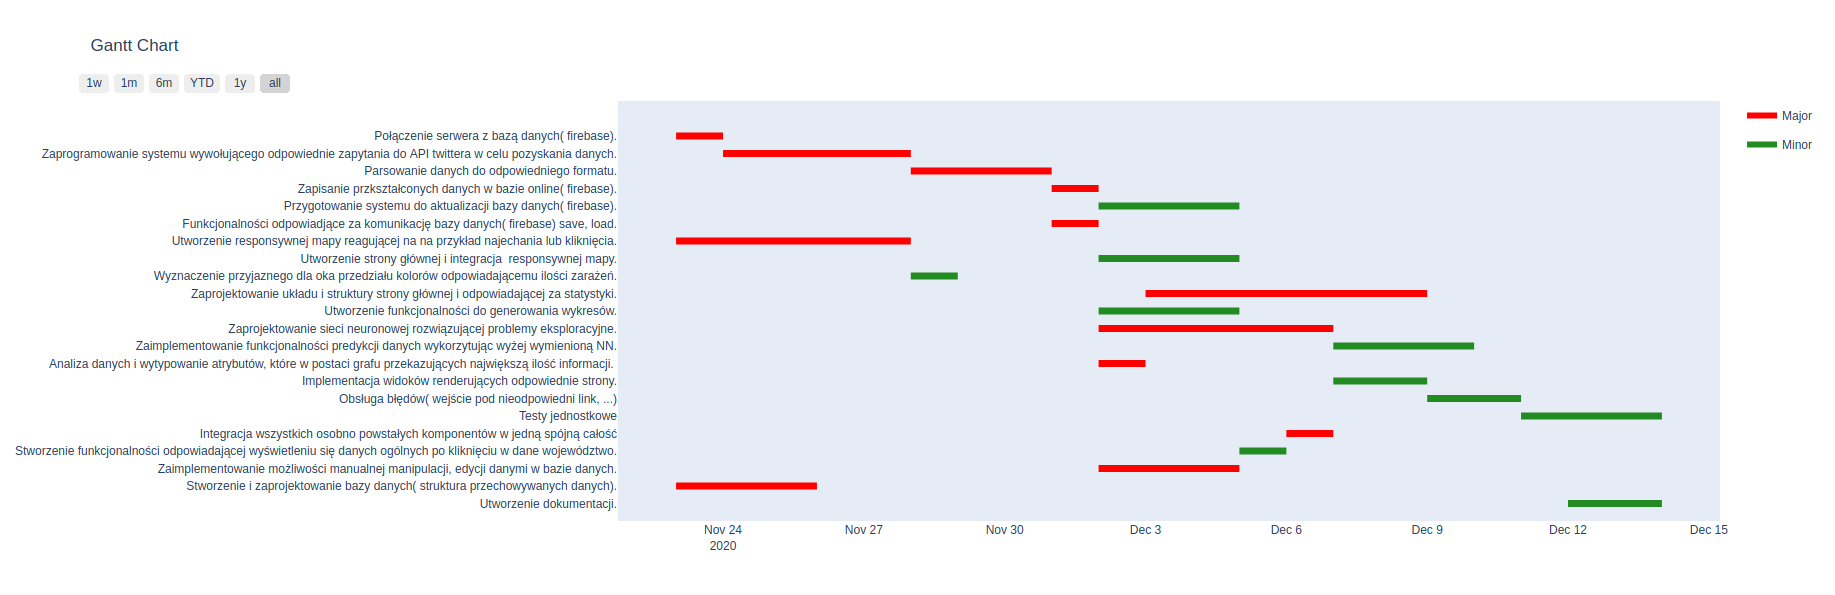
\includegraphics[scale=0.3]{gantt.png}
\end{figure}
\section{Opis cech charakterystycznych technologii wybranych do realizacji projektu oraz uzasadnienie, dla-
czego powinny one zostać użyte w projekcie.}


\begin{enumerate}
\item {\bf Firebase}- baza danych online pozwala na aktualizowanie danych z dowolnego miejsca. Jeśli jakikolwiek użytkownik spróbuje połączyć się z naszą aplikacją nasze dane zostana zaktualizowane niezależnie od miejsca i urządzenia. \\Kolejnym atutem użycia takiej technologii jest to, że pozwola nam ona na przechowywanie danych do generowania wykresów czy diagramów.
\item {\bf Django}- pośredniczy w komunikacji klient serwer. Odpowiada za operacje nad bazą danych, przekazywanie danych i renderowanie odpowiednich template'ów.
\item {\bf HTML}- korzystamy z jego "pudełkowej" struktury do grupowania i uporządkowania elementów naszej strony.
\item {\bf CSS}- pozwala na odpowiednia koloryzację, dodanie atrybutów, pozycjonowanie.
\item {\bf Javascript}- jest potrzebny do utworzenia pewnych dynamicznych zachowań na naszej stronie na przykład do utworzenia mapy, wykorzystujemy go do dynamicznego zmieniania pewnych cech elementów pod wpływem jakiegoś działania na przykład przesunięcia paska.
\item {\bf canvasJS, chartJS} Generowanie wykresów, diagramów w sekcji statystyki, ogólna wizualizacja danych.
\item {\bf tweepy} Wrapper do api twittera, wykorzystywany do pobierania danych z ofcijalnego konta ministerstwa zdrowia
\end{enumerate}
\end{document}